% do not change these two lines (this is a hard requirement
% there is one exception: you might replace oneside by twoside in case you deliver 
% the printed version in the accordant format
\documentclass[11pt,titlepage,oneside,openany]{article}
\usepackage{times}

\usepackage{url}
\usepackage[hidelinks]{hyperref}
\usepackage{wrapfig}
\usepackage{graphicx}
\usepackage{latexsym}
\usepackage{amsmath}
\usepackage{amssymb}
\usepackage{listings}

\usepackage{ntheorem}

% \usepackage{paralist}
\usepackage{tabularx}

% this packaes are useful for nice algorithms
\usepackage{algorithm}
\usepackage{algorithmic}

% well, when your work is concerned with definitions, proposition and so on, we suggest this
% feel free to add Corrolary, Theorem or whatever you need
\newtheorem{definition}{Definition}
\newtheorem{proposition}{Proposition}


% its always useful to have some shortcuts (some are specific for algorithms
% if you do not like your formating you can change it here (instead of scanning through the whole text)
\renewcommand{\algorithmiccomment}[1]{\ensuremath{\rhd} \textit{#1}}
\def\MYCALL#1#2{{\small\textsc{#1}}(\textup{#2})}
\def\MYSET#1{\scshape{#1}}
\def\MYAND{\textbf{ and }}
\def\MYOR{\textbf{ or }}
\def\MYNOT{\textbf{ not }}
\def\MYTHROW{\textbf{ throw }}
\def\MYBREAK{\textbf{break }}
\def\MYEXCEPT#1{\scshape{#1}}
\def\MYTO{\textbf{ to }}
\def\MYNIL{\textsc{Nil}}
\def\MYUNKNOWN{ unknown }
% simple stuff (not all of this is used in this examples thesis
\def\INT{{\mathcal I}} % interpretation
\def\ONT{{\mathcal O}} % ontology
\def\SEM{{\mathcal S}} % alignment semantic
\def\ALI{{\mathcal A}} % alignment
\def\USE{{\mathcal U}} % set of unsatisfiable entities
\def\CON{{\mathcal C}} % conflict set
\def\DIA{\Delta} % diagnosis
% mups and mips
\def\MUP{{\mathcal M}} % ontology
\def\MIP{{\mathcal M}} % ontology
% distributed and local entities
\newcommand{\cc}[2]{\mathit{#1}\hspace{-1pt} \# \hspace{-1pt} \mathit{#2}}
\newcommand{\cx}[1]{\mathit{#1}}
% complex stuff
\def\MER#1#2#3#4{#1 \cup_{#3}^{#2} #4} % merged ontology
\def\MUPALL#1#2#3#4#5{\textit{MUPS}_{#1}\left(#2, #3, #4, #5\right)} % the set of all mups for some concept
\def\MIPALL#1#2{\textit{MIPS}_{#1}\left(#2\right)} % the set of all mips





\begin{document}

\pagenumbering{roman}
% lets go for the title page, something like this should be okay
\begin{titlepage}
	\vspace*{2cm}
  \begin{center}
   {\Large IE650 Semantic Web Technologies\\}
   \vspace{2cm} 
   {Project Report\\}
   \vspace{2cm}
   {presented by\\
    Oliver Frendo (1510432) \\
    Sascha Ulbrich (1493181) \\
   }
   \vspace{1cm} 
   {submitted to the\\
    Data and Web Science Group\\
    Prof.\ Dr.\ Paulheim\\
    University of Mannheim\\} \vspace{2cm}
   {December 2016}
  \end{center}
\end{titlepage} 

% no lets make some add some table of contents
\tableofcontents
\newpage

%\listofalgorithms

%\listoffigures

%\listoftables

% evntuelly you might add something like this
% \listtheorems{definition}
% \listtheorems{proposition}

\newpage


% okay, start new numbering ... here is where it really starts
\pagenumbering{arabic}

%• 10-12 pages (sharp!) without title and toc pages 
%• due Friday, December 2nd, 23:59 
%• send by email to Anna Lisa, André and Heiko 
%• describe your solution including the steps to get there (chapters already created)

%Requirements 
%You must use the DWS master thesis layout
%Please cite sources properly. Preferred citation style [Author, year]





\section{Application domain and goals}
The goal of this application is to allow a user browsing websites to automatically retrieve additional information about entities in a given text. The information should be presented to the user in a way that is easily consumable. 

As such this application targets any user that is interested in supplementary information while browsing. By automating the process of looking up entities the user saves time as he does not have to manually visit other websites such as Wikipedia. 

In addition, the application searches for information in many sources. This way the information does not stem from any one source but is the union of several sources.  During search the application retrieves only certain attributes. These attributes can be customized by the user, thus allowing him to decide which information should be retrieved. The application will focus on English input to simplify processing.



 %Olli
\section{Datasets used} 
\label{sec:datasets}
In order to identify as many named entities as possible with one source we started with the DBpedia dataset \cite{dbpedia_dbpedia_2016}
using the public data endpoint\footnote{\url{http://dbpedia.org/sparql}} and tested with the corresponding Virtuoso \cite{openlink_software_openlink_2016} SPARQL explorer\footnote{\url{http://dbpedia.org/snorql/}}.

As such a first version of the application was focused on querying DBpedia only. In later versions query generation was refactored such that it can be used for all sources supporting SPARQL 1.1. The technical details are described in the next section. Per source only the endpoint URL as well as the source specific RDF Type URIs for organisations, locations and persons have to be specified, e.g. \textit{http://dbpedia.org/ontology/Organisation} for DBpedia. This information is needed to incorporate the entity type information retrieved from the named entity recognitions and as filter for entity search. The filter serves two purposes: performance is increased because only labels of entities of this type are considered for matching the name and to increase the chance to find the correct entity, assuming that the retrieved entity type is correct. 

The application offers a configurable set of sources to request entities from as described in table \ref{tab:sources}.

\begin{table}[H]
	\begin{tabular*}{\textwidth}{p{2,2cm}|p{3,8cm}|p{2,1cm} |p{3cm}}
		
		\textbf{Data Set} &\small \textbf{SPARQL Endpoint} & \textbf{Entities} & \textbf{Usage}  \\
		\hline 
		\textbf{DBpediaLive} &\small \url{http://dbpedia-live.openlinksw.com/sparql/} & Organisation, Person, Location  & Active per default\\
		\hline 
		\textbf{iServer} &\small \url{http://iserve.kmi.open.ac.uk/iserve/sparql} & Organisation & Active per default \\
		\hline 
		\textbf{FactForge} &\small \url{http://factforge.net/sparql} & Organisation, Person, Location & Error: Timeout \\
		\hline 
		\textbf{European Environment Agency} &\small \url{http://semantic.eea.europa.eu/sparql} &  Organisation, Person, Location  & Error: only supports SPARQL 1.0  \\
		\hline   
		\textbf{LinkedMDB} &\small \url{http://linkedmdb.org/sparql} &  Organisation, Person, Location  & Error: only supports SPARQL 1.0 \\
		\hline 
		\textbf{Education (UK)} & \small \url{http://services.data.gov.uk/education/sparql} &  Organisation, Location  & Slow, and sameAs definitions are missing \\
		\hline 
		\textbf{DataGov (UK)} &\small \url{http://services.data.gov.uk/reference/sparql} &  Organisation, Person  & Not useful, only internal links\\
		\hline 
		\textbf{World Bank} &\small \url{http://worldbank.270a.info/sparql} &  Location & Error: No rdfs:label, uses skos:prefLabel \\
		\hline 
		\textbf{YAGO2} &\small \url{https://linkeddata1.calcul.u-psud.fr/sparql} &  Organisation, Person, Location & Active per default, but slowest \\
	\end{tabular*}
	\caption{Additional data sources and their usage}
	\label{tab:sources}
\end{table}

Most of the source were identified via a webpage called ''SPARQL Endpoints Status'' \cite{pierre-yves_vandenbussche_sparql_2013}. This website monitors hundreds of SPARQL endpoints, allows the user to filter based on interoperability (SPARQL 1.1) and provides an availability chart. This helped a lot to judge whether or not a endpoint could be usable from a technical point of view. Afterwards the data source was explored by selecting the available RDF types and searching for potentially interesting properties. 















 %Sascha
\section{Techniques used} 

\subsection{Overview}
%Olli
This section describes the techniques that were used to implement the application. Figure \ref{fig:architecture} shows the architecture. The main components are the Chrome browser in which the Chrome extension is installed, a Java server to handle input and output and a set of sources, each of which has its own SPARQL endpoint. 


\begin{figure}[ht]
	\centering
	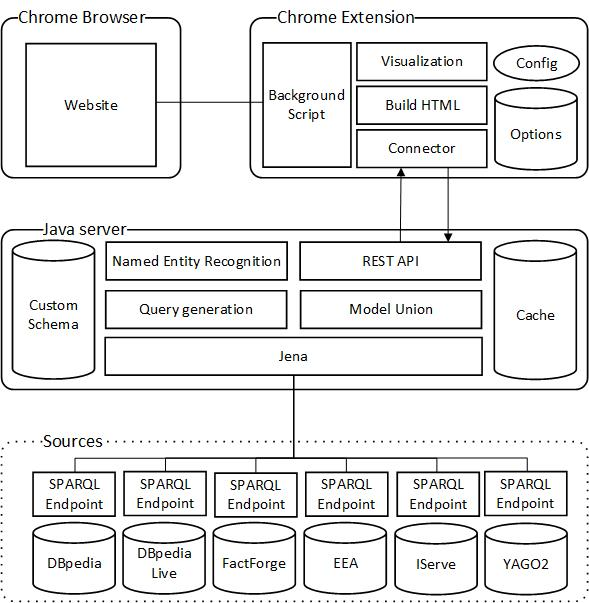
\includegraphics[width=0.8\textwidth]{img/Architecture_v2}
	\caption{Architecture}
	\label{fig:architecture}
\end{figure}


%Reasoning
%Search
%external services
%
%Server
%Chrome extension


\subsection{Named Entity Recognition}
%Olli
Named entity recognition (NER) was used to implement a process that receives as input free text and produces as output a set of named entities \cite{NERTutorial}. Stanford's CoreNLP\footnote{\url{http://stanfordnlp.github.io/CoreNLP/}} was used to implement this. First, the input is cleansed by tokenizing, applying Part-of-Speech tags and lemmatization. Next NER is applied. 

The intermediate result is a set of annotated tokens. To retrieve entities specifically tokens of the type \textit{PERSON}, \textit{LOCATION} and \textit{ORGANIZATION} are used. Other types such as \textit{MISC}, \textit{DATE} or \textit{NUMBER} are ignored \cite{CoreNLP_NER}. The final step is to make sure entities consisting of multiple words, e.g. names, are not retrieved as individual entities. To implement this the tokens are processed sequentially and concatenated as long as they are annotated with the same type. 

For example, the sentence ``Passenger Ruby Gupta, 20, was travelling to Azamagarh to be married on 1 December.'' should produce two entities \texttt{Ruby Gupta} (\textit{PERSON}) and \texttt{Azamagarh} (\textit{LOCATION}) but not an entity \texttt{1 December} (\textit{DATE}). The set of annotated tokens is shown in figure \ref{fig:nerExample}. 

 \begin{figure}[ht]
	\centering
	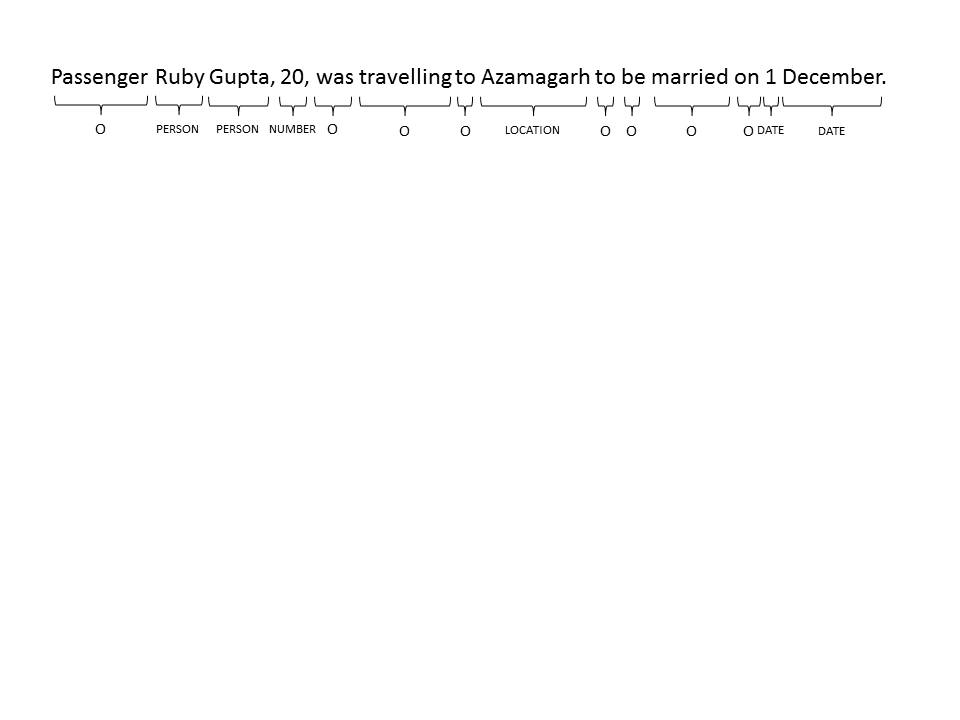
\includegraphics[width=0.8\textwidth]{img/nerExample}
	\caption{Sample NER-annotated text}
	\label{fig:nerExample}
\end{figure}
 




\subsection{SPARQL Queries}
\label{sec:sparqlQueries}
%Sascha
After identifying the named entity and its entity type these information are handed over to the query engine which is implemented using Jena\footnote{\url{https://jena.apache.org/}}. The query process is divided into two steps, first all selected sources are queried in parallel in own threads and afterwards after all are finished the results are merged into one model where the result properties and the context triples are derived from. These two steps are illustrated in Figure \ref{fig:details_query} and explained in more detail in the following.
\begin{figure}[ht]
	\centering
	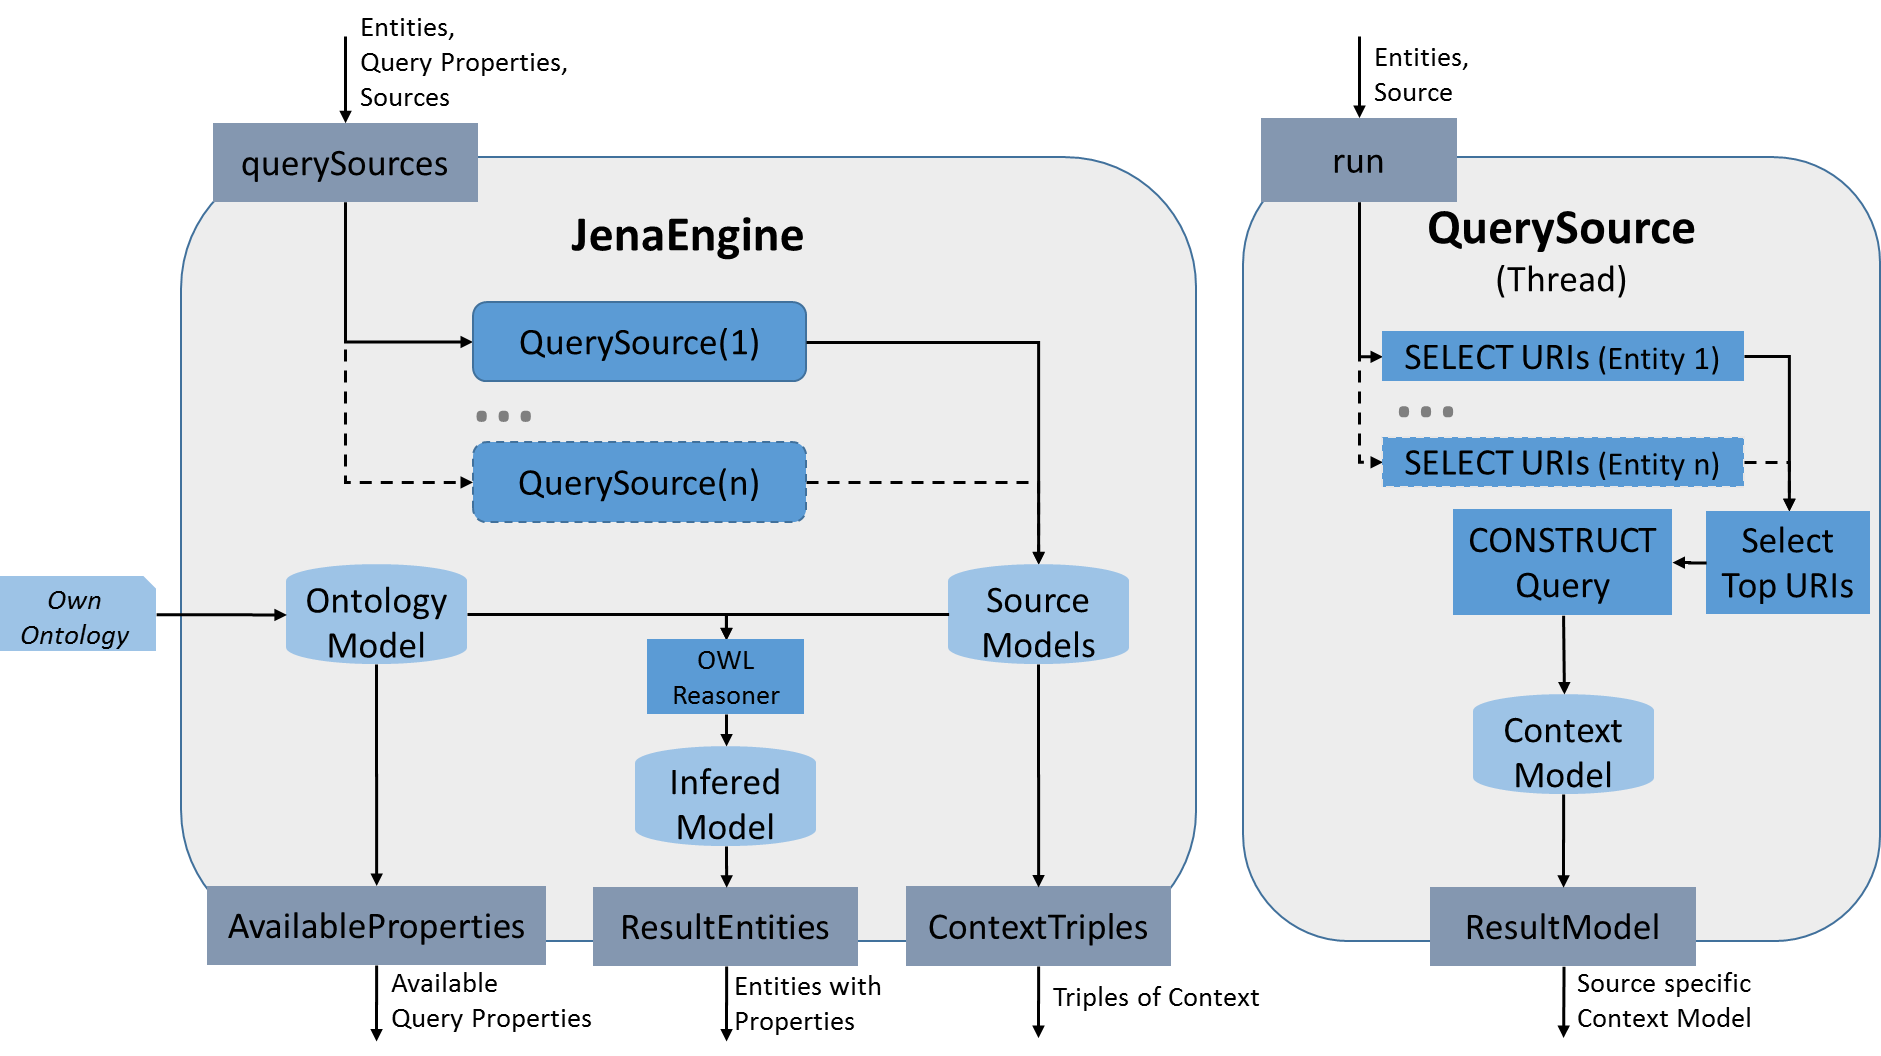
\includegraphics[width=1\textwidth]{img/QueryEngineDetails}
	\caption{Details of Query Engine}
	\label{fig:details_query}
\end{figure}

\paragraph{Querying Sources}
All sources are queried the same way via class QuerySource as illustrated in Figure \ref{fig:details_query} on the right hand side. Source queries could be generalized since the only differences are the endpoint URLs and entity type URIs as described before. In order to derive properties and context of a source based on the names and types of the entities, multiple queries are executed in two steps.

First step is the identification of URI candidates by performing a reg-ex based search per identified entity in the context. These queries run in parallel so the system can handle multiple entities without significant increase in runtime. Technically multiple \textit{SELECT-Queries} are executed, as shown in Figure \ref{fig:details_query}. The results of these first queries are URIs which meet the type definition and the reg-ex. The reg-ex allows up to 10 characters before and after the identified name and a period is replaces with ".*" to allow a match with shortened names. In cases there are too many matches (currently the threshold is five), an extended logic is used to reduce the amount of URI candidates. 

The approach for URI selection is based on a score which is calculated for each URI by multiplying a \textit{relation score} and the normalized edit distance of the URI label and the entity name. Therefore the source queries provide a count of relations available per URI. This information is used to calculate the \textit{relation score}, which is a relative score, being 1 for the URI with the most relations. The top five URIs with the highest score are selected. Less URIs are selected if there are not enough URIs having at least a score value of at least 75\% of the highest score value.

In a second step the identified URI candidates are used to query the source specific context. So all properties are queried as well as direct and in-direct relations between the entities. Furthermore the labels of all elements are derived as well as OWL \textit{sameAs} relations. 
This last query is a \textit{Construct-Query} and therefore returns a model which is the result of the source queries, as shown in Figure \ref{fig:details_query}. 

\paragraph{Querying Local Model}
After all source queries are finished the derived models are added to the same local model, as illustrated in Figure \ref{fig:details_query} on the left hand side. This model is combined with an own ontology defined for this project. This own ontology mainly consists of OWL \textit{euivelantProperty} definitions for own properties which group the corresponding sources specific properties. Furthermore there is a mapping of own classes representing the entity types to the corresponding source specific class definitions of the entities. Therefore the OWL \textit{equivalentClass} property is used. For inference the \textit{OWLMicroReasoner} is used. More complex OWL reasoner need much more time, so they are not used for performance reasons. 

Before the properties are derived from this inferred model, one URI per entity is derived across sources. The one with most relations is chosen. 
For these URIs the properties are then queried based on the own ontology and returned as result. If there are multiple result values for a property all values are returned. If the same value occurs multiple times for the same property, a count is increased. For numeric values additional logic is applied to ensure proper formatting and unit references. All property values including a language tag which is not empty nor English are discarded.


\subsection{Server} 
\label{sec:server}
%Olli
The server's role in the application is to act as middleware between the frontend and the components that generate and handle SPARQL queries. It implements a REST API with two calls: GET /RetrieveAvailableProperties and POST /RetrieveTriples. All inputs and outputs are communicated via JSON. The first call is used by the frontend to allow the user to view which attributes are available. The second call retrieves a set of triples for a given text. Examples for both can be viewed in \texttt{README.md}\footnote{\url{https://github.com/ofrendo/SemanticWebTechnologies/}}. 

Lastly, the server must implement HTTPS. This is because the user may view websites available only over HTTPS and browsers do not allow mixed content, i.e. loading resources over HTTP on an HTTPS website \cite{ChromeMixedContent}. To achieve this the first idea was to use Heroku for cloud hosting\footnote{\url{https://www.heroku.com/}}. This would ensure that the server is always available and it automatically offers a secure connection. However, it quickly turned out that the server used more memory than was allowed on Heroku (1GB). As such it was decided to use a local server instead. To ensure a secure connection a small server (nginx) with a reverse proxy was used with self signed certificates\cite{nginxReverseProxy}. 




\subsection{Chrome extension}
%Olli
The Chrome extension handles communication to and from the server and shows the result to the user. It consists mainly of a content script\footnote{\url{https://developer.chrome.com/extensions/content_scripts}}, which is a JavaScript file that is loaded on every website. Upon loading it injects an HTML button that starts the process when clicked. 

\begin{wrapfigure}{h}{5.5cm}
  \frame{
	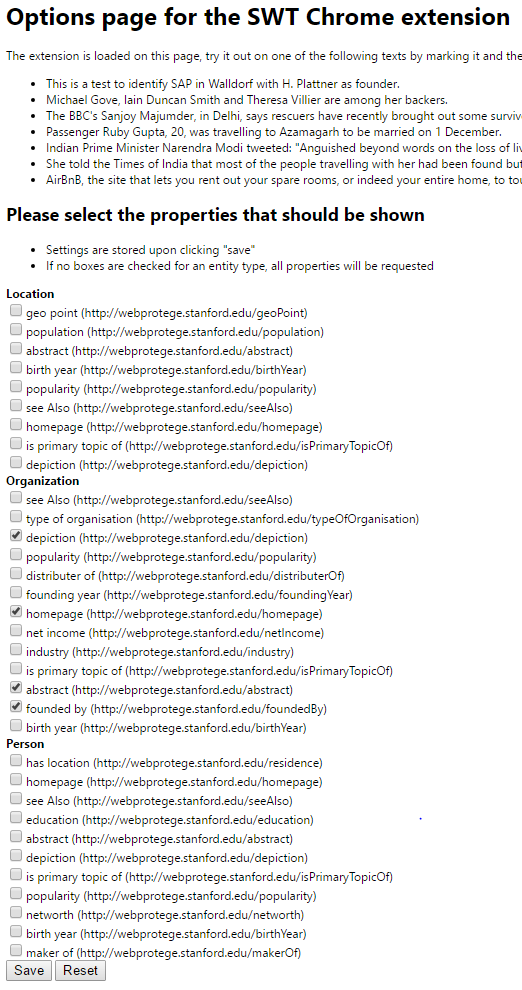
\includegraphics[width=5.5cm]{img/sampleResults/options} %1\textwidth
  }
  \caption{Options page}
  \label{fig:options}
\end{wrapfigure}

\paragraph{Loading triples}
If the user has marked any text on the website this is used as input for the second API call. After the HTTP request has finished loading a popup showing the results is generated and injected into the website. A section is built for each entity showing the triples that were retrieved. Any duplicates are removed. Values with the same relation type (e.g. \textit{abstract}) are compared to each other with the Jaccard similarity measure. If the similarity crosses a threshold the values are hidden as similar attributes. The user can view the attributes by clicking on them if he wishes to. We treated further methods of data fusion, such as trying out other similarity measures, as out of scope, as described in the project outline. 




\paragraph{Options}
The user has the possibility to customize which attributes are retrieved. For this an options page\footnote{\url{https://developer.chrome.com/extensions/options}} was implemented. This page first loads the available properties via GET /RetrieveAvailableProperties and then shows the results to the user (see figure \ref{fig:options}). The user selects the attributes he is interested in and saves them locally. Any subsequent queries send these options along with the input text. Besides allowing the user to customize the application and reducing bandwith another benefit is that it may also improve query execution time. 


\paragraph{Visualization}
%TODO: first order connections - is that described above?
The second API call (POST /RetrieveTriples) retrieves a set of context triples as described in section \ref{sec:sparqlQueries}. These are visualized to show the user the connections between entities. The visualization is generated by D3.js \footnote{\url{https://d3js.org/}} and a force layout. 































 % both
\section{Example results}
%Olli

Figure \ref{fig:sampleResults} shows some screenshots from the Chrome extension. In it, the user is browsing Spiegel and has selected some text (see A on the left side). After clicking ``Search for entities'', the popup on the right appears with additional information about entities in the marked text. In this case, two entities \texttt{Merkel} (see A and B) and Germany (see C) have been found. For \texttt{Merkel}, several similar values for \textit{abstract} have been found (see B at the bottom). These can be expanded by clicking. The last picture (D) visualizes the connections between the two entities. Big circles (orange and purple) represent subjects and objects of triples while the smaller circles (light blue) represent the names of relations. 



\begin{figure}[H]
	\centering
	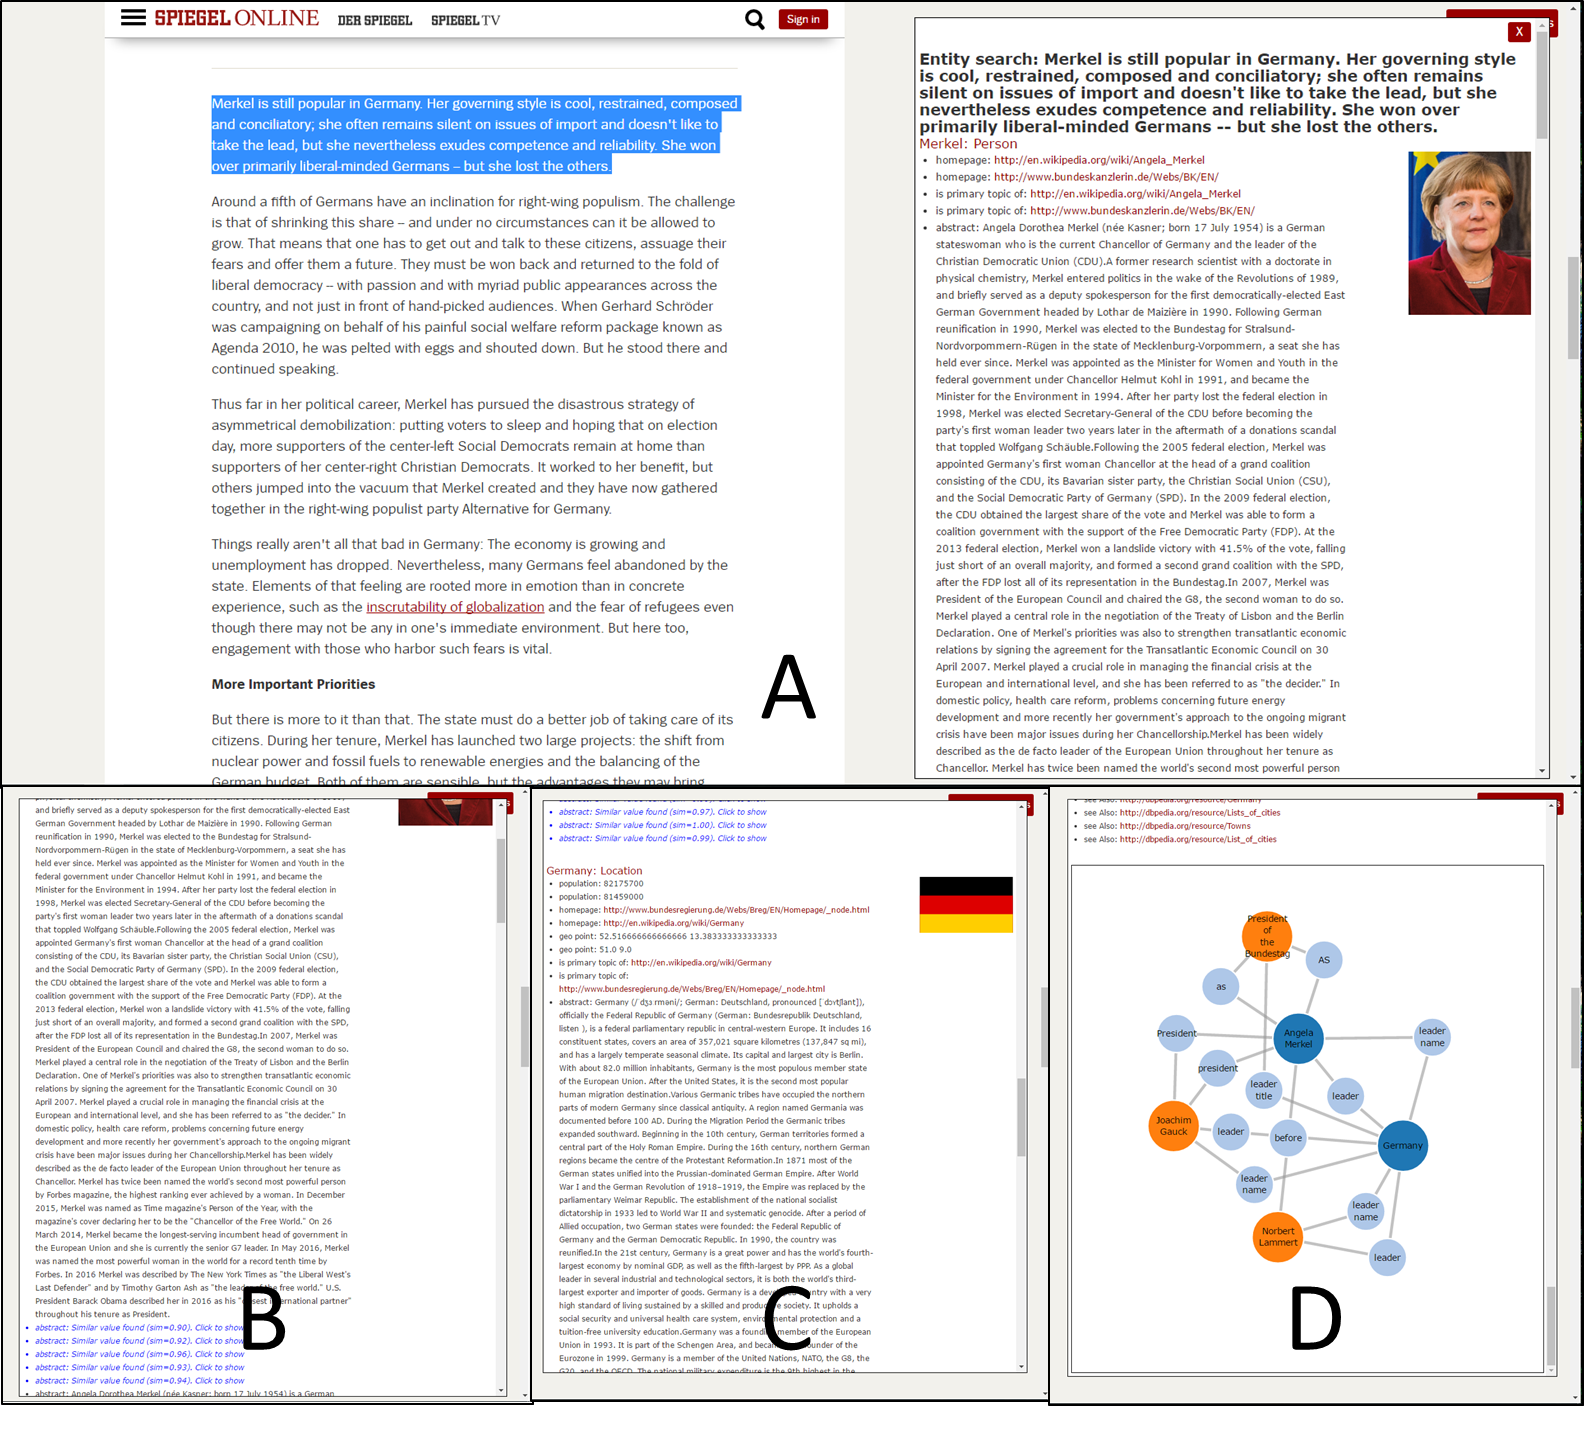
\includegraphics[width=1\textwidth]{img/sampleResults/sampleResult}
	\caption{Sample result}
	\label{fig:sampleResults}
\end{figure}






 %Olli
\section{Known limitations}
In which domains does the application not work? 
- other languages



Are there queries which cannot be answered? – Why? 
- queries with too many entities (i.e. long text): waiting time very high
- memory limitations






How could you overcome those limitations, given more time?
- Cache commonly requested entities locally (in a TBA)
- Another limitation: self signed certificate. Given more time: Instead of running the server locally, host the server on the internet and set up a domain redirecting to the IP adress of the server and buying/setting up a secure certificate for the domain


We could mention papers describing techniques which could improve certain areas like LINDA \cite{boehm_linda:_2012} for entity matching. 


 %both
\section{Lessons learned}
\subsection{Working with SPARQL Endpoints}
One of the main obstacles was working with different SPARQL endpoints, because they use different ways to express the same knowledge. Often, the SPARQL endpoints themselves were a source of trouble. DBpedia was a good starting point even though it is sometimes not available or slow. Well functioning and known public endpoints are quite occupied. As such a reasonable mechanism of these endpoints is to reject execution of queries if the estimated runtime is too long. However, it was very interesting to play around with the SPARQL explorer and learn in this way how to use SPARQL and its limitations. Sometimes the query just needed to be reformulated a bit such that the query could be optimized better\footnote{as describe at \url{https://github.com/openlink/virtuoso-opensource/issues/28}}.

As described in section \ref{sec:sparqlQueries} the URI identification turned out to be the most expensive part. Because of this  these queries were formulated to be as efficient as possible and to be executed in parallel. As soon as URIs are identified more complex queries are possible. That makes sense since the regex-based search of URIs requires parsing a large set of labels. In contrast URIs could be accessed directly if indexed properly. This means formulating the queries for URI search in a way which is not rejected by the endpoint and is as performant as possible was one of the biggest obstacles. In this context some fine tuning was necessary as well in order to optimize the matches of the reg-ex-pattern and special handling for example of locations because they often contain further region information like ``Rochester, New York''. This was solved with the previously described extended logic including a similarity score for URI labels. Incorporating this logic into SPARQL queries was not possible, because of complexity. 

Furthermore many SPARQL endpoints are not active anymore or do not support SPARQL 1.1. As such searching for potentially useful SPARQL endpoints was focused on technical aspects first. As described in section \ref{sec:datasets} multiple endpoints have been integrated. But some turned out to not be useful, for example the ones hosted by the UK government services. These sources do not contain OWL \textit{sameAs} definitions and therefore could not be matched.

\subsection{Chrome Extension}
One of the challenges for the Chrome extension was implementing it to be reusable on every website. Injecting HTML on every site is straightforward but ensuring that it looks the same is more challenging because each website has its own CSS rules.

A solution for this could be to use a different method for the chrome extension. Instead of injecting HTML popups \footnote{\url{https://developer.chrome.com/extensions/browserAction\#popups}} could be used for display. This way the extension has the same look and feel on every website because it is independent of it. The downside of this is that a connection between the popup and the website the user is currently on could be hard to implement. A workaround could be for the user to copy and paste input text into a box in the popup. 

Another issue was finding a good way to visualize connections between entities, conceptually as well as technically. It was decided that implementing a visualization of the graph within the application was too time consuming, which was why d3.js was used to create the visualization.




\subsection{Potential Improvements and Outlook}
For a productive solution hosting the datasets and using them via private SPARQL endpoints would be necessary in order to offer a stable service. This should not only improve stability but should reduce query runtime as well. Scalability of the application should be quite good since the most expensive part is already cached. 
In order to stay flexible the integration of external/public services should still be possible. But the process should be adapted in order to minimize impact of slow sources on the runtime, as this is a limitation describe in section \ref{sec:Limits}. This could be solved by providing partial results to the end-user which are updated while the query processes are ongoing. A good example for such an approach is the FactForge RelFinder\footnote{\url{http://factforge.net/relfinder}}. Furthermore the ability to specify sources to be queried could be integrated in the options for the end user in order to allow manual (temporary) disabling of certain sources. 

Furthermore the links between datasets in terms of OWL \textit{sameAs} definitions could be enriched by performing entity matching across sources (similar to LINDA \cite{boehm_linda:_2012}). Since this process needs to run automated it could also be a potential source of failure. 

Lastly, another aspect is the extensibility. The custom ontology is already customizable via an ontology file. But the source specification is hard coded which could be easily exchanged with a configuration via a configuration file defining the endpoint and the specific entity type URIs. 



 %both










%References
%Add own references in .bib file
\pagebreak
\bibliographystyle{apalike}
\bibliography{SWTReport_Sascha,SWTReport_Olli}


\end{document}
